\documentclass[12pt,a4paper]{article}
\usepackage[utf8]{inputenc}%Para Tildes y ñ%
\usepackage[spanish]{babel}
\usepackage{amsmath}
\usepackage{amsfonts}
\usepackage{amssymb}
\usepackage{siunitx}
\usepackage{adjustbox}
%\usepackage{minted}
\usepackage[american]{circuitikz}
\usepackage{tikz}
\usepackage{graphicx} 
\usepackage{pdfpages} %para importar paginas de un pdf 
\usepackage{booktabs}
\usepackage{multicol}
\usepackage[bookmarks = true, colorlinks=true, linkcolor = black, citecolor = green, menucolor = black, urlcolor = black]{hyperref} 
\usepackage[left=2cm,right=2cm,top=2cm,bottom=2cm]{geometry} 
\usepackage{multirow}
\addto\captionsspanish{\renewcommand{\listtablename}{Índice de tablas}}		% Cambiar nombre a lista de tablas   
\addto\captionsspanish{\renewcommand{\tablename}{Tabla}}					% Cambiar nombre a tablas
\usepackage{float}		% Para ubicar las tablas y figuras justo después del texto
\usepackage{pdfpages}
\usepackage{enumerate}%listas y viñetas
\author{Estudiantes:\\ Kevin Campos Castro\\ Josué Salmerón Córdoba  \\{\small Grupo 1}\\ Profesor:  Marco Villalta  \vspace*{3.0in}}
\title{Universidad de Costa Rica\\{\small Facultad de Ingeniería\\Escuela de Ingeniería Eléctrica\\IE0624 - Proyecto\\III ciclo 2023\\\vspace*{0.55in}}\\ Título: Smart Door Lock \vspace*{1.35in}}
%\date{fecha de entrega} 

\begin{document} 

\maketitle  
\thispagestyle{empty}%%no numerar la portada
\renewcommand{\thepage}{\roman{page}}
\newpage
\tableofcontents
\newpage
\listoffigures 
\newpage
\listoftables  
\newpage
%%%%%%%%%%  
\renewcommand{\thepage}{\arabic{page}} 
\setcounter{page}{1}
\begin{center}
\section{Resumen}
\end{center}
% AQUI VA EL RESUMEN 
Este trabajo se implementó un smart door lock que consta de dos cerraduras y está dividivo en las siguientes secciones. En la primera se hace uso de TinyML con un Arduino Nano 33 Ble Sense para el reconocimiento de voz. La segunda sección se hace uso de un microcontrolador Arduino Mega2560 un keypad, una pantalla lcd para una mejorar interacción con el usuario. Ambas secciones tienen un servo motor en común y se encargarán de realizar la misma tarea, es decir, abrir y cerrar la puerta de dos maneras distintas. Donde se obtuvieron los resultados esperados cumpliendo satisfactoriamente los objetivos del proyecto.

   
\newpage  


\section{Objetivos}
\subsection{Objetivos General}
\begin{itemize}
\item Crear un sistema inteligente que permita abrir y cerrar una puerta por medio de un Keypad y voz.

\end{itemize}

\subsection{Objetivos Específicos}
\begin{itemize}
\item Implementar el uso de TinyML con Edge Impulse para grabar las palabras claves.
\item Encender LEDs para indicar el estado de la puerta (abierta o cerrada).
\item Implementación de periféricos como keypad, servo, pantalla LCD para poder abrir la puerta de forma manual.
\end{itemize} 
\newpage

\section{Alcances}
Las limitaciones de este proyecto fueron las siguientes:
\begin{itemize}
\item Los materiales disponibles para la construcción de la puerta no fueron los mejores, son muy pesados y no tan portátiles en transporte público.
\item Haber tenido una pequeña noción de la existencia de Edge Impulse al inicio del curso hubiese sido de gran ayuda ya que el proyecto estaba para más aplicaciones como el reconocimiento facial.
\item Realizar un entrenamiento más estricto, esto incluye cantidad de muestras, diferentes voces en distintas horas del día.
\item El costo total es bien alto debido al uso de dos placas, esto pudo haberse evitado con el hecho de haber revisado el funcionamiento del Arduino Nano Ble 33 Sense con más anticipación.
\end{itemize}
\section{Justificación}
La razón por la que se decidió realizar este proyecto se basa en la necesidad de crear un prototipo de caja fuerte inteligente que pueda ser desbloqueada tanto por comandos de voz como manualmente a través de un keypad. Esta combinación de métodos de acceso aumenta la comodidad y la accesibilidad para una variedad de personas, esto incluye a personas que tienen sus manos ocupadas en dicho momento o personas con limitaciones físicas que se les dificulta el ingreso de una clave convencional.
Además, el proyecto ayuda ampliar nuestro conocimiento y experiencia en el manejo de componentes físicos, como el keypad, el servo y la pantalla LCD (aunque esta última fue simulada pero no implementada). El proceso de trabajar con estos periféricos no solo fortalece nuestra comprensión de la electrónica y la programación, sino que también nos prepara para abordar proyectos más complejos en el futuro, donde la integración de múltiples dispositivos será fundamental.
Por último, la implementación de machine learning en un MCU es un aprendizaje de gran valor para futuros proyectos porque permite explorar aplicaciones que van más allá de las soluciones convencionales, abriendo nuevas posibilidades en el diseño y la implementación de sistemas inteligentes y adaptativos. 
\section{Nota teórica}
\subsection*{Arduino Nano 33 Ble Sense}
El arduino Nano 33 BLE Sense es un módulo miniatura que contiene un módulo NINA B306, basado en Nordic nRF52480 y contiene un M4F Cortex, un cripto chip el cual puede almacenar certificados de forma segura y pre-compartir llaves y un IMU de 9 ejes. El módulo puede ser montado como un componente DIP o como componente SMT, directamente soldado por la vía de los pads. Es importante mencionar que la parte de TinyML forma parte de este proyecto, ya que implica reconocimiento de voz, por tanto, hay entrenamiento previo con la grabación de las acciones que se desean realizar, es decir, abrir y cerrar más dos complementos adicionales como sonidos desconocidos y ruido esto porque un modelo de ML no tiene idea sobre las cosas que están bien o mal, y solo aprende con los datos que se le dan, en ese sentido, entre más variado sean los datos, el modelo trabajará mejor \cite{web5}. Ahora, también es importante mencionar que la librería PDM y el sensor MP34DT05 ayudaron a la captura de las muestras esto porque los micrófonos se encargan de hacer la conversión de de sonidos en datos digitales.
\begin{figure}[H]
\centering
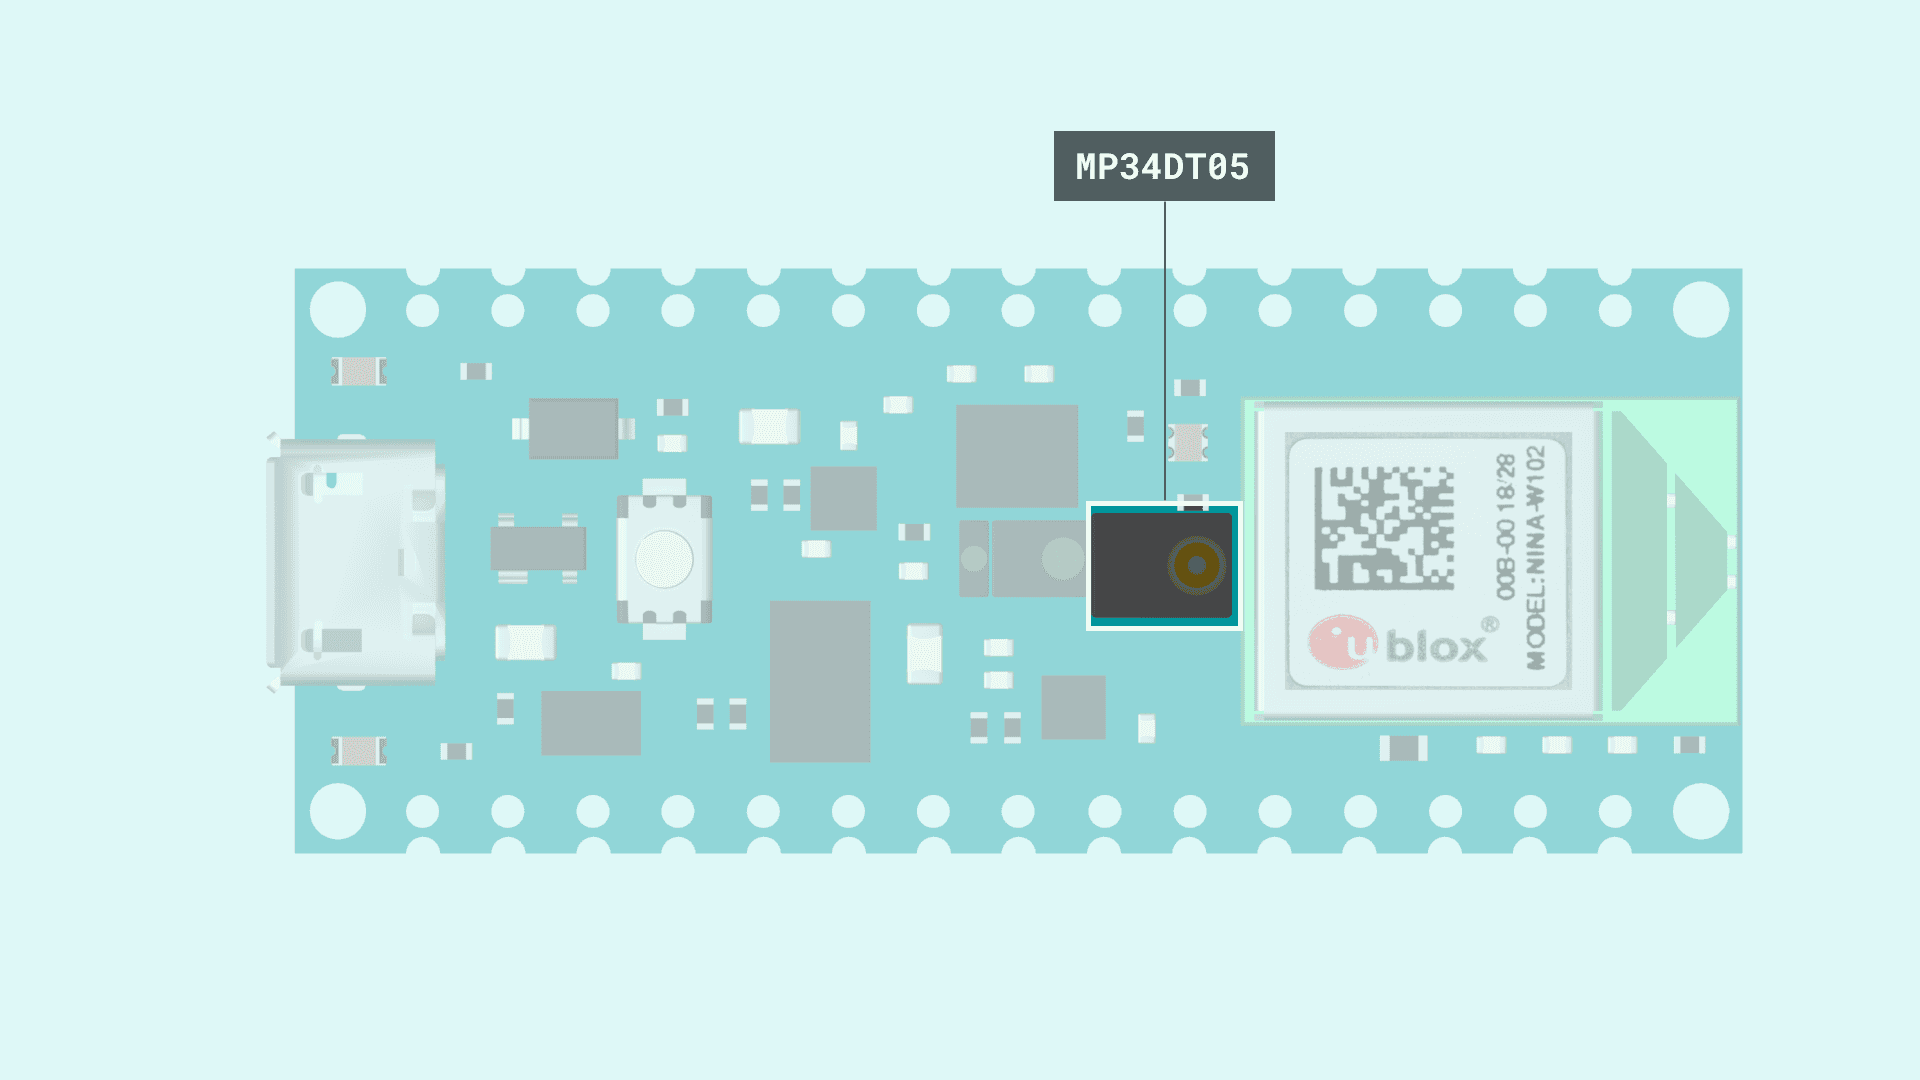
\includegraphics[width=.55\linewidth]{Img/Nano33_ble_sense_microphone.png}
 \caption{Ubicación del micrófono. Tomado de \cite{web6}.}
 \label{fig_micro}
\end{figure}


\subsubsection*{Características generales}
Las características más importantes de este mcu se mencionan a continuación \cite{web}
\begin{multicols}{2}
 \begin{itemize}
    \item CPU: ARM Cortex-M4 a 64MHz con FPU, 32-bit, 1MB Flash, 256kB SRAM.
    \item Bluetooth 5, IEEE 802.15.4-2006, \SI{2.4}{\giga\Hz}.
    \item ARM TrusZone Cryptocell 310 security subsystem, secure boot.
    \item USB 2.0, QSPI, SPI.
    \item 48 GPIOs.
    \item 12-bit, ADC con 8 canales.
    \item 64 comparadores de nivel, 15 del tipo low-power.
    \item Sensor de temperatura.
    \item $4\times4$-canales PWM.
    \item Periféricos de audio: I2S, PDM
    \item $5\times32$-bit timers.
    \item $4\times$ SPI maestros\/$3\times$ SPI esclavos.
    \item $2\times$I2C.
    \item $2\times$ UART.
    \item decodificador de cuadratura (QDEC).
    \item $3\times$ RTC.
\end{itemize}   
\end{multicols}

\subsubsection*{Diagrama de bloques}
La figura \ref{fig1} representa el diagrama de bloques de la placa.
\begin{figure}[H]
\centering
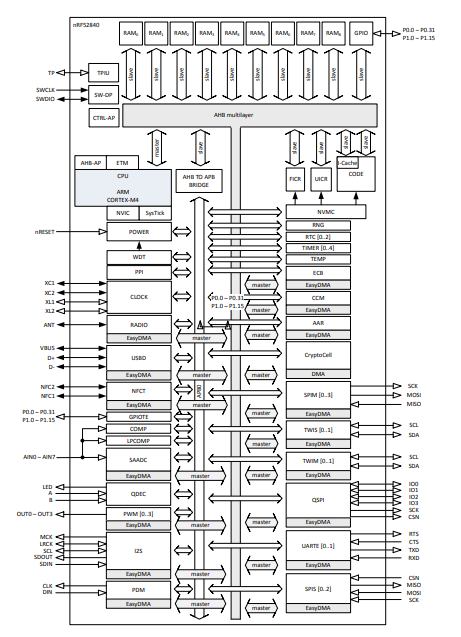
\includegraphics[width=.55\linewidth]{Img/1.png}
 \caption{Diagrama de bloques del Nano BLE 33 Sense . Tomado de \cite{web}.}
 \label{fig1} 
\end{figure}
\newpage
\subsubsection*{Diagrama de pines}
El diagrama de la figura \ref{fig2} brinda de manera más detallada la distribución de los pines.
\begin{figure}[H]
\centering
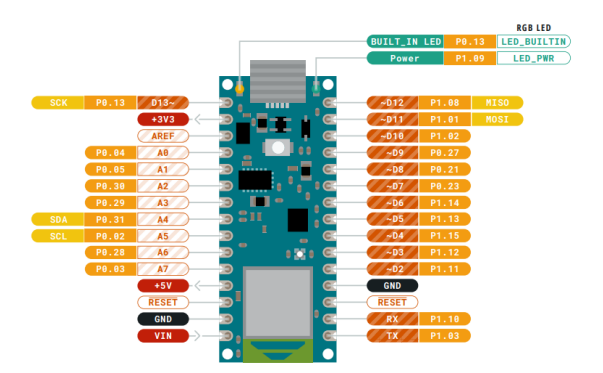
\includegraphics[width=.55\linewidth]{Img/2.png}
 \caption{Diagrama de pines del Nano BLE 33 Sense . Tomado de \cite{web2}.}
 \label{fig2}
\end{figure}

\subsubsection*{Características eléctricas}
Aquí se tomaron dos referencias para tener más claro este detalle,  primero se muestran los valores máximos del mcu nRF52480 y los de la placa respectivamente.
\begin{figure}[H]
\centering
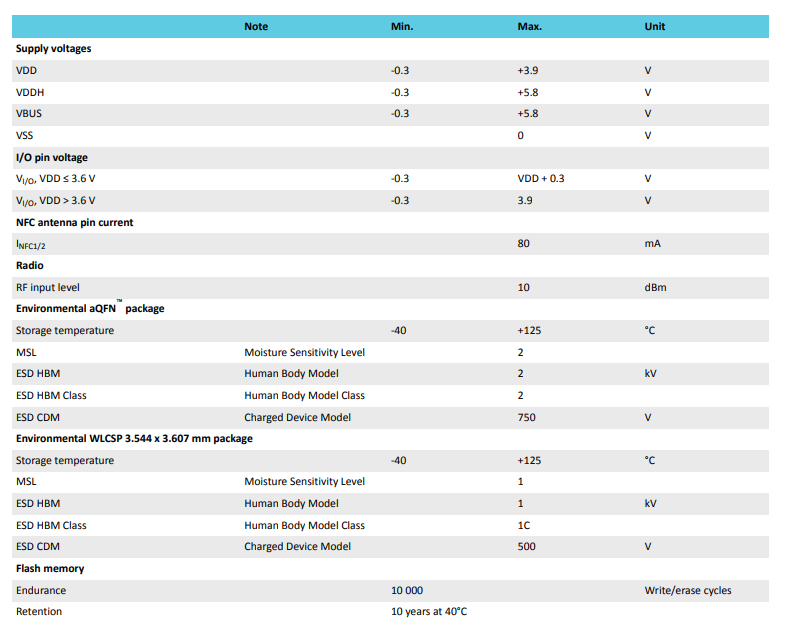
\includegraphics[width=.55\linewidth]{Img/3.png}
 \caption{Características eléctricas de nRF52480. Tomado de \cite{web}.}
 \label{fig3}
\end{figure}

\begin{figure}[H]
\centering
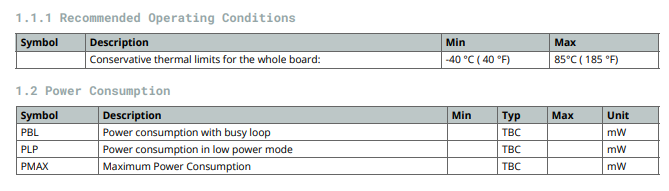
\includegraphics[width=.55\linewidth]{Img/3.1.png}
 \caption{ Características eléctricas de la placa. Tomado de \cite{web2}.}
 \label{fig3.1}
\end{figure}

%%%%%%%%%%%%%%%%%%%%%%%%%%%%%%%%%%% Arduino Atmega
\subsection*{Arduino Mega 2560 Rev3}
El verdadero MCU utilizado es el elegoo MEGA 2560 R3, sin embargo comparte las mismas características que el arduino, la documentación de esta última está más depurada es por esta razón que fue la que se tomó como base.

\subsubsection{Características generales}
Las características generales de este MCU se describe a continuación \cite{ArduinoMega}:
\begin{itemize}
    \item Rendimiento de hasta 16 MIPS a 16 MHz
    \item 256k bytes (de los cuales 8k se utilizan para el cargador de arranque)
    \item 4k bytes EEPROM
    \item 8k bytes de SRAM interna
    \item 32 × 8 registros de trabajo de propósito general
    \item Contador en tiempo real con oscilador separado
    \item Cuatro canales PWM de 8 bits
    \item Cuatro USART serie programables
    \item Interfaz serie SPI controladora/periférica
\end{itemize}

\subsubsection{Diagrama de bloques}
\begin{figure}[H]
    \centering
    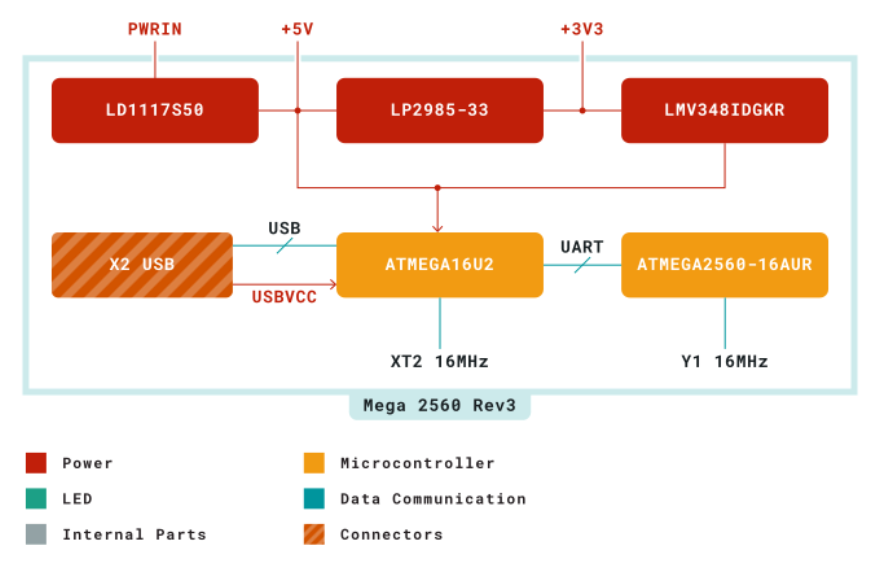
\includegraphics[width=.6\linewidth]{Img/k1.png}
    \caption{ Diagrama de bloques del arduino mega 2560 REV3 \cite{ArduinoMega}.}
\end{figure}

\subsubsection{Diagrama de pines}
\begin{figure}[H]
    \centering
    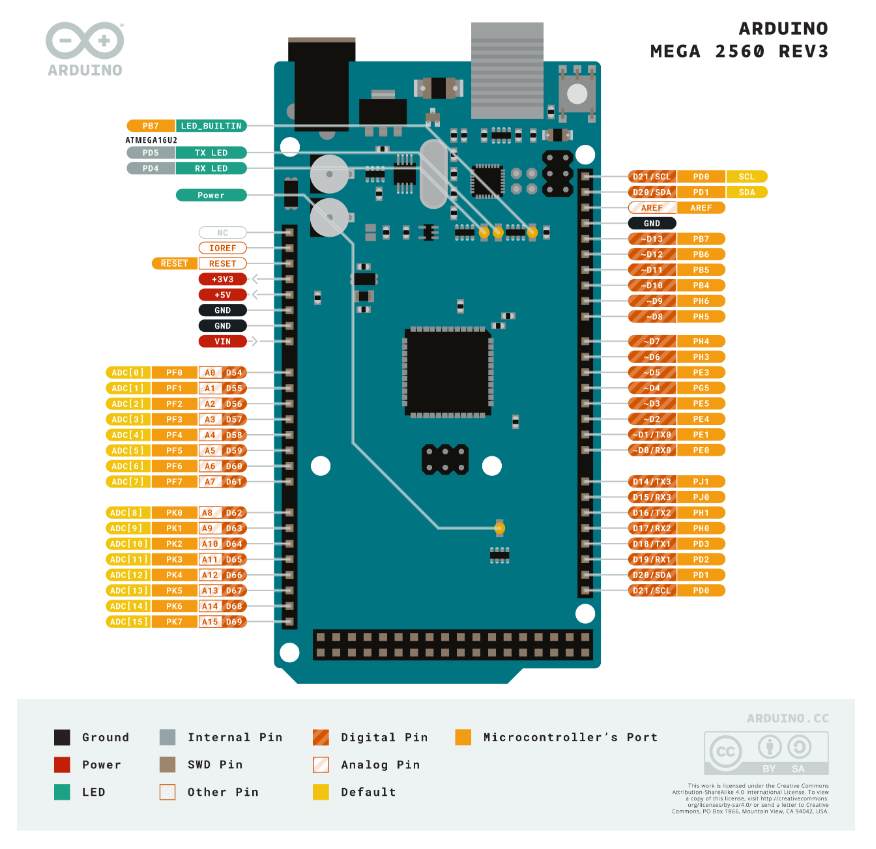
\includegraphics[width=.6\linewidth]{Img/k2.png}
    \caption{ Diagrama de pines del arduino mega 2560 REV3 \cite{ArduinoMega}.}
\end{figure}

\subsubsection{Características eléctricas}
\begin{figure}[H]
    \centering
    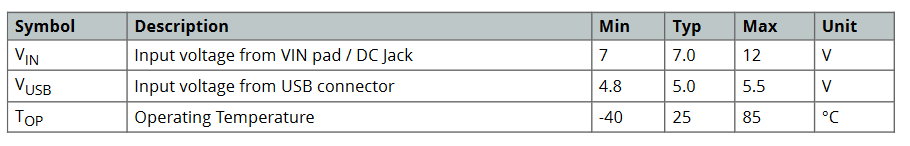
\includegraphics[width=.6\linewidth]{Img/k3.png}
    \caption{ Condiciones de operación del arduino mega 2560 REV3 \cite{ArduinoMega}.}
\end{figure}

\subsection*{Periféricos utilizados}
Los principales periféricos para este proyecto fueron el módulo I2C y el sensor MP34DT05.\par
% Escribir algo de teoría de I2C.
La idea de usar este módulo es incorporarlo con la pantalla lcd porque facilita la conexión con el arduino Mega2560 por lo que solo basta con conectar los pines \texttt{GND},\texttt{VCC},\texttt{SDA} y \texttt{SCL} de la figura \ref{fig_i2c}, donde los dos últimos tienen que ver los datos seriales y el reloj. Donde una condición de parada: alto-bajo corresponde a la transición SDA (I/O) mientras que SCL está en alto y es enviada por el \texttt{master}. Otro detalle es que estos pines necesitan resistencias de pull-up apropiadas y tomar en consideración la capacitancia total de todos los esclavos del bus I$^2$C. Los dos primeros pines se trata de una conexión básica, fuente a tierra y la alimentación del módulo que esto va conectado con los \SI{5}{\volt} del arduino Mega2560 \cite{web8}.\par
Por otro lado, el sensor MP34DT05 es un micrófono ultra-compacto que usa PDM (modulación densidad de pulso) para representar una señal analógica como una señal binaria. El rango del sensor posee diferentes valores:
\begin{itemize}
    \item Radio señal de ruido: \SI{64}{\dB}.
    \item Sensibilidad: $-26\text{dBFS} \pm \SI{3}{\dB} $
    \item Rango de temperatura: -40 a $\SI{85}{\celsius}$
\end{itemize}

\subsection*{Componentes electrónicos complementarios}
En función de cumplir con los objetivos del proyecto los siguientes componentes fueron de gran ayuda para cumplirlos.
\subsubsection*{Keypad}
La función del Keypad es para escribir la clave que se mostrará en la pantalla lcd.
\begin{figure}[H]
    \centering
    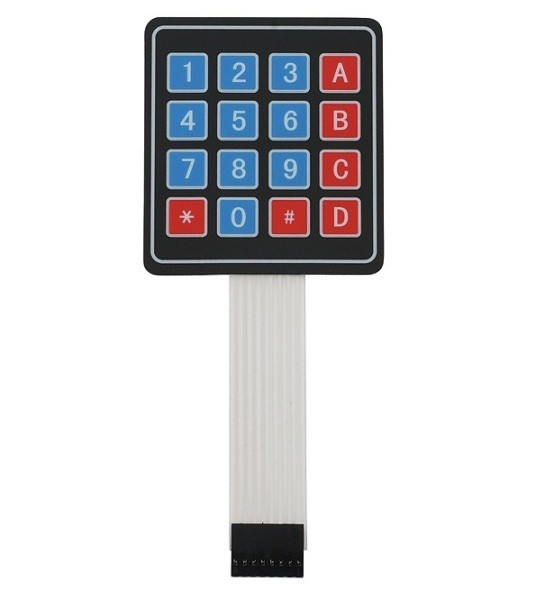
\includegraphics[width=.4\linewidth]{Img/keypad.jpg}
    \caption{Keypad}
    \label{fig_keypad}
\end{figure}
\subsubsection*{Módulo I2C}
Este componente es sumamente importante porque se incorpora a la pantalla lcd para establecer la comunicación con el microcontrolador y luego con el keypad.
\begin{figure}[H]
    \centering
    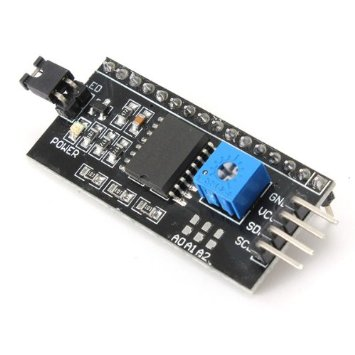
\includegraphics[width=.4\linewidth]{Img/i2c.jpg}
    \caption{Módulo I2C.}
    \label{fig_i2c}
\end{figure}
\subsubsection*{Pantalla lcd}
Su tarea es mostrar la entrada del usuario, si escribe la contraseña correcta o incorrecta se mostrará un mensaje en la pantalla.
\begin{figure}[H]
    \centering
    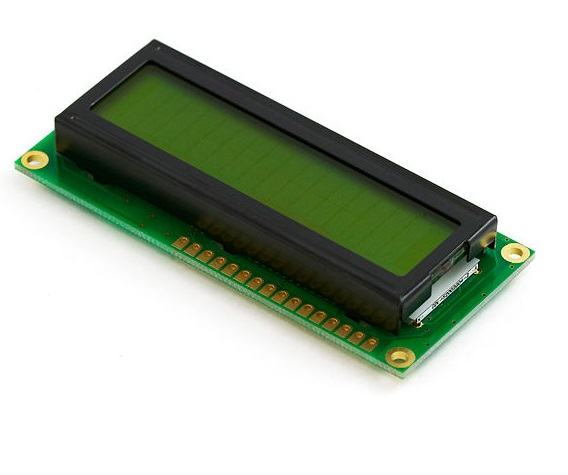
\includegraphics[width=.4\linewidth]{Img/lcd.jpg}
    \caption{Pantalla lcd.}
    \label{fig_lcd}
\end{figure}
\subsubsection*{Servomotor}
Este componente se encarga de abrir o cerrar la puerta dependiendo de dos aspectos. El primero es con la clave escrita en el keypad y lo segundo con base a las palabras claves: \textit{abrir} o \textit{cierra}.
\begin{figure}[H]
    \centering
    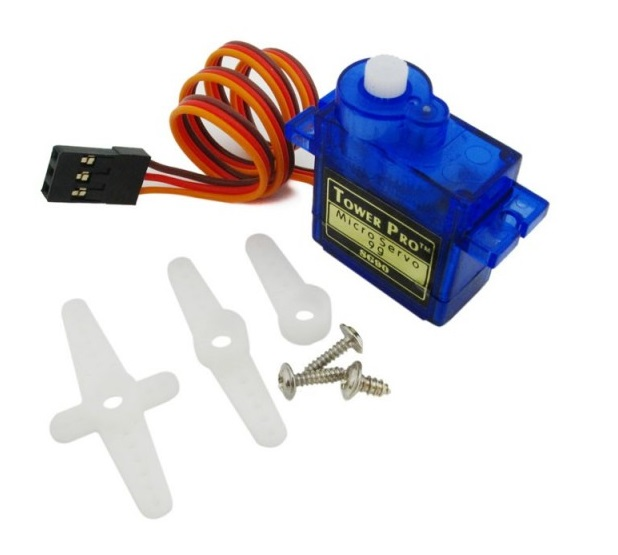
\includegraphics[width=.4\linewidth]{Img/servo.jpg}
    \caption{Servomotor.}
    \label{fig_servo}
\end{figure}
Ahora, por medio de muchas pruebas realizadas se determinó que no fue posible trabajar solo con el Arduino Nano 33 Ble Sense ya que se determinó en el laboratorio que el pin de \SI{5}{\volt} no funcionaba porque mostraba una salida de \SI{5}{\volt}. El otro problema que se mostró fue a la hora de hacer la conexión con el keypad porque a la hora de presionar cualquier botón por medio del monitor serial se estaban reconociendo caracteres completamente desconocidos, ante esto se diseñó un filtro RC en la salida, esto para las pulsaciones, sin embargo, el problema persistía. El otro problema es con la pantalla lcd, ella necesita una alimentación de al menos \SI{5}{\volt}, en ese sentido debe estar conectada a un pin que posee esa salida, de lo contrario muestra un bajo contraste y no se puede apreciar correctamente el contenido, para solucionar este problema pudo haberse hecho un par Darlington o realizar lo mostrado en la figura \ref{fig_usb}.

\begin{figure}[H]
    \centering
    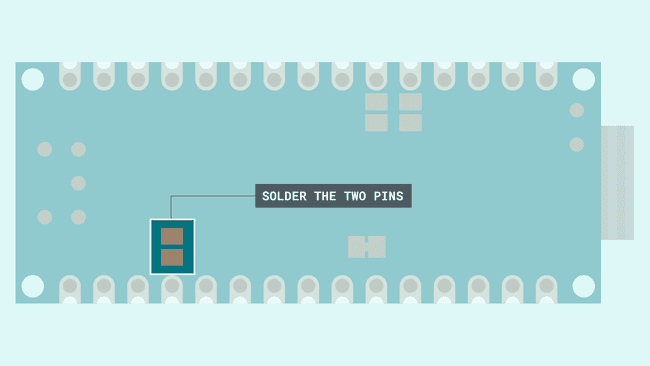
\includegraphics[width=.4\linewidth]{Img/pin_vusb.png}
    \caption{Habilitación de \SI{5}{\volt}.}
    \label{fig_usb}
\end{figure}
No obstante, por cuestiones de tiempo y complejidad en ese tipo de soldadura especial/fina no se tomaron esos caminos. Ante todos estas situaciones lo más favorable fue hacer uso de otra placa para realizar estas conexiones. Entonces, el proyecto tiene dos etapas:
\begin{itemize}
    \item La placa Arduino MEGA2560, se encarga de abrir y cerrar la puerta por medio del keypad cuando se le escribe la contraseña correcta y controlar el display.
    \item La placa Arduino Nano 33 Ble Sense fue entrenada con 4 clases; dos keywords (abrir/cerrar) y otras dos con ruido y sonidos desconocidos. Así, cuando reconozca alguna de las palabras claves se abrirá o cerrará la puerta y encenderá un LED dependiendo del estado.
\end{itemize}

% TABLA DE COMPONENTES
\begin{table}[H]
\caption{Lista de equipos}
\label{table_2}
\begin{center}
\begin{tabular}{r|cc}
\hline
\textbf{Componente}&\textbf{Cantidad}&\textbf{Precio}\\
 \hline
Arduino Nano 33 Ble Sense& 1 &60\$ \\ \hline 
Arduino Mega2560& 1 & 18\$ \\ \hline 
Keypad& 1 &9\$ \\ \hline 
Pantalla lcd& 1 &6.95\$ \\ \hline 
Servomotor& 2 &11\$ \\ \hline 
Batería \SI{9}{\volt}& 1 &5.5\$ \\ \hline 
Kit de resistencias& 1 & 0.2\$ \\ \hline 
Kit de jumpers & 1 &2 \$ \\ \hline 
Módulo I2C & 1 & 4\$ \\ \hline 

 \textbf{Total}& & 117\$ \\
 \hline
\end{tabular}
\end{center}
\end{table}

\subsection*{Diseño del circuito}
\begin{figure}[H]
    \centering
\tikzset{every picture/.style={line width=0.75pt}} %set default line width to 0.75pt        

\begin{tikzpicture}[x=0.75pt,y=0.75pt,yscale=-1,xscale=1]
%uncomment if require: \path (0,649); %set diagram left start at 0, and has height of 649

%Flowchart: Connector [id:dp42585090626324207] 
\draw   (304,59) .. controls (304,44.64) and (315.64,33) .. (330,33) .. controls (344.36,33) and (356,44.64) .. (356,59) .. controls (356,73.36) and (344.36,85) .. (330,85) .. controls (315.64,85) and (304,73.36) .. (304,59) -- cycle ;
%Straight Lines [id:da9927818650372262] 
\draw    (329.92,85) -- (329.92,101) ;
\draw [shift={(329.92,104)}, rotate = 270] [fill={rgb, 255:red, 0; green, 0; blue, 0 }  ][line width=0.08]  [draw opacity=0] (8.93,-4.29) -- (0,0) -- (8.93,4.29) -- cycle    ;
%Flowchart: Decision [id:dp8222109791046812] 
\draw   (334.92,223) -- (393.17,267) -- (334.92,311) -- (276.67,267) -- cycle ;
%Shape: Right Angle [id:dp5468713947182464] 
\draw   (276.67,267) -- (251,267) -- (251,302) ;
%Straight Lines [id:da34123972616362797] 
\draw    (251,302) -- (251.87,322) ;
\draw [shift={(252,325)}, rotate = 267.51] [fill={rgb, 255:red, 0; green, 0; blue, 0 }  ][line width=0.08]  [draw opacity=0] (8.93,-4.29) -- (0,0) -- (8.93,4.29) -- cycle    ;
%Flowchart: Process [id:dp6422094052668206] 
\draw   (208,323) -- (297,323) -- (297,361) -- (208,361) -- cycle ;
%Shape: Right Angle [id:dp9632380337734168] 
\draw   (393.17,267) -- (419,267) -- (419,299) ;
%Straight Lines [id:da9224648988654192] 
\draw    (419,299) -- (419.87,319) ;
\draw [shift={(420,322)}, rotate = 267.51] [fill={rgb, 255:red, 0; green, 0; blue, 0 }  ][line width=0.08]  [draw opacity=0] (8.93,-4.29) -- (0,0) -- (8.93,4.29) -- cycle    ;
%Straight Lines [id:da14093121348085114] 
\draw    (424,375) -- (423.23,410) ;
\draw [shift={(423.17,413)}, rotate = 271.26] [fill={rgb, 255:red, 0; green, 0; blue, 0 }  ][line width=0.08]  [draw opacity=0] (8.93,-4.29) -- (0,0) -- (8.93,4.29) -- cycle    ;
%Flowchart: Connector [id:dp28231580529895073] 
\draw   (143,571) .. controls (143,556.64) and (154.64,545) .. (169,545) .. controls (183.36,545) and (195,556.64) .. (195,571) .. controls (195,585.36) and (183.36,597) .. (169,597) .. controls (154.64,597) and (143,585.36) .. (143,571) -- cycle ;
%Flowchart: Document [id:dp7887811718871025] 
\draw   (373,321) -- (470,321) -- (470,368.85) .. controls (409.38,368.85) and (421.5,386.1) .. (373,374.94) -- cycle ;
%Shape: Right Angle [id:dp7465732461480319] 
\draw   (449.17,439) -- (487,439) -- (487,185) ;
%Straight Lines [id:da9427213356074324] 
\draw    (384,184.03) -- (487,185) ;
\draw [shift={(381,184)}, rotate = 0.54] [fill={rgb, 255:red, 0; green, 0; blue, 0 }  ][line width=0.08]  [draw opacity=0] (8.93,-4.29) -- (0,0) -- (8.93,4.29) -- cycle    ;
%Flowchart: Connector [id:dp6793358076053446] 
\draw   (397.17,439) .. controls (397.17,424.64) and (408.81,413) .. (423.17,413) .. controls (437.53,413) and (449.17,424.64) .. (449.17,439) .. controls (449.17,453.36) and (437.53,465) .. (423.17,465) .. controls (408.81,465) and (397.17,453.36) .. (397.17,439) -- cycle ;
%Straight Lines [id:da6157101498528812] 
\draw    (253,361) -- (253.87,381) ;
\draw [shift={(254,384)}, rotate = 267.51] [fill={rgb, 255:red, 0; green, 0; blue, 0 }  ][line width=0.08]  [draw opacity=0] (8.93,-4.29) -- (0,0) -- (8.93,4.29) -- cycle    ;
%Flowchart: Process [id:dp10984865947746725] 
\draw   (296,481) -- (385,481) -- (385,519) -- (296,519) -- cycle ;
%Flowchart: Process [id:dp2789359345260862] 
\draw   (287,105) -- (376,105) -- (376,143) -- (287,143) -- cycle ;
%Straight Lines [id:da14083283346218511] 
\draw    (334,201) -- (334.87,221) ;
\draw [shift={(335,224)}, rotate = 267.51] [fill={rgb, 255:red, 0; green, 0; blue, 0 }  ][line width=0.08]  [draw opacity=0] (8.93,-4.29) -- (0,0) -- (8.93,4.29) -- cycle    ;
%Flowchart: Decision [id:dp06088544865395984] 
\draw   (254,384) -- (312.25,428) -- (254,472) -- (195.75,428) -- cycle ;
%Shape: Right Angle [id:dp8217099184396621] 
\draw   (313.17,428) -- (339,428) -- (339,460) ;
%Straight Lines [id:da965375327404175] 
\draw    (339,460) -- (339.87,480) ;
\draw [shift={(340,483)}, rotate = 267.51] [fill={rgb, 255:red, 0; green, 0; blue, 0 }  ][line width=0.08]  [draw opacity=0] (8.93,-4.29) -- (0,0) -- (8.93,4.29) -- cycle    ;
%Shape: Right Angle [id:dp7886934725142394] 
\draw   (195.67,429) -- (170,429) -- (170,464) ;
%Straight Lines [id:da8518021831322284] 
\draw    (170,464) -- (170.87,484) ;
\draw [shift={(171,487)}, rotate = 267.51] [fill={rgb, 255:red, 0; green, 0; blue, 0 }  ][line width=0.08]  [draw opacity=0] (8.93,-4.29) -- (0,0) -- (8.93,4.29) -- cycle    ;
%Flowchart: Process [id:dp8640224184714345] 
\draw   (127,488) -- (216,488) -- (216,526) -- (127,526) -- cycle ;
%Shape: Right Angle [id:dp5762038720241354] 
\draw   (383,504) -- (422,504) -- (422,483) ;
%Straight Lines [id:da6437862550472608] 
\draw    (422,483) -- (422.97,467.99) ;
\draw [shift={(423.17,465)}, rotate = 93.71] [fill={rgb, 255:red, 0; green, 0; blue, 0 }  ][line width=0.08]  [draw opacity=0] (10.72,-5.15) -- (0,0) -- (10.72,5.15) -- (7.12,0) -- cycle    ;
%Flowchart: Document [id:dp3979180887556457] 
\draw   (288,167) -- (381,167) -- (381,196.7) .. controls (322.88,196.7) and (334.5,207.41) .. (288,200.48) -- cycle ;
%Straight Lines [id:da5018025676967481] 
\draw    (331,144) -- (331.87,164) ;
\draw [shift={(332,167)}, rotate = 267.51] [fill={rgb, 255:red, 0; green, 0; blue, 0 }  ][line width=0.08]  [draw opacity=0] (8.93,-4.29) -- (0,0) -- (8.93,4.29) -- cycle    ;
%Straight Lines [id:da6767101156206579] 
\draw    (169,525) -- (169,542) ;
\draw [shift={(169,545)}, rotate = 270] [fill={rgb, 255:red, 0; green, 0; blue, 0 }  ][line width=0.08]  [draw opacity=0] (8.93,-4.29) -- (0,0) -- (8.93,4.29) -- cycle    ;

% Text Node
\draw (313,49) node [anchor=north west][inner sep=0.75pt]   [align=left] {Inicio};
% Text Node
\draw (250.92,244) node [anchor=north west][inner sep=0.75pt]   [align=left] {Si};
% Text Node
\draw (212.08,332.67) node [anchor=north west][inner sep=0.75pt]   [align=left] {Abre puerta};
% Text Node
\draw (311,241) node [anchor=north west][inner sep=0.75pt]   [align=left] {Clave\\correcta\\};
% Text Node
\draw (401.92,247) node [anchor=north west][inner sep=0.75pt]   [align=left] {No};
% Text Node
\draw (161,561) node [anchor=north west][inner sep=0.75pt]   [align=left] {fin};
% Text Node
\draw (377.08,326.67) node [anchor=north west][inner sep=0.75pt]   [align=left] {clave\\incorrecta};
% Text Node
\draw (300.08,490.67) node [anchor=north west][inner sep=0.75pt]   [align=left] {puerta=0};
% Text Node
\draw (298.08,114.67) node [anchor=north west][inner sep=0.75pt]   [align=left] { puerta=0};
% Text Node
\draw (219,418) node [anchor=north west][inner sep=0.75pt]   [align=left] {puerta==90};
% Text Node
\draw (321.92,408) node [anchor=north west][inner sep=0.75pt]   [align=left] {No};
% Text Node
\draw (169.92,406) node [anchor=north west][inner sep=0.75pt]   [align=left] {Si};
% Text Node
\draw (135.08,497.67) node [anchor=north west][inner sep=0.75pt]   [align=left] {puerta=90};
% Text Node
\draw (296.08,173.67) node [anchor=north west][inner sep=0.75pt]   [align=left] {Digite clave};


\end{tikzpicture}

    \caption{Diagrama de bloques smart door lock.}
    \label{sch_1}
\end{figure}
El diagrama mostrado anteriormente es la lógica que posee el proyecto en general. Gracias a este esquema, desde un inicio se tuvo claro los objetivos a cumplir.
%\newpage

\section{Desarrollo/Análisis}
Inicialmente se hicieron todas las configuraciones necesarios con las referencias\cite{web5} dadas en clase. Hecho esto se logró sincronizar el microcontrolador con la página Edge Impulse. Esto permitió hacer uso del micrófono del Arduino Nano Ble 33 Sense y así comenzar con las grabaciones.

\begin{figure}[H]
\centering
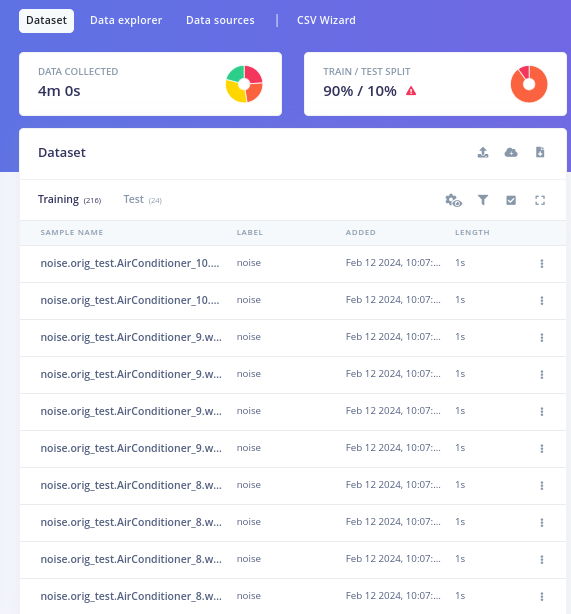
\includegraphics[width=.55\linewidth]{Img/data_set.png}
 \caption{Conjunto de datos.}
 \label{fig_dataset}
\end{figure}
En total de 240 muestras clasificadas por etiquetas.
\begin{itemize}
\item \texttt{OPEN\_TAG}.
    \begin{figure}[H]
    \centering
    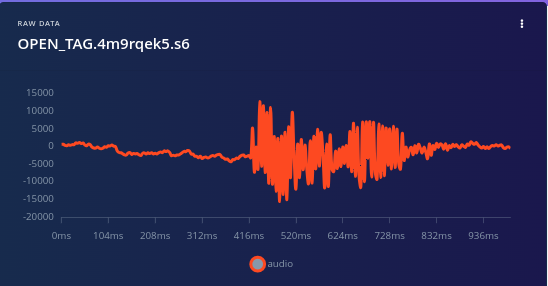
\includegraphics[width=.4\linewidth]{Img/open_tag.png}
    \caption{Espectro señal abrir.}
    \label{open_tag}
    \end{figure}
\item \texttt{CLOSE\_TAG}.
     \begin{figure}[H]
    \centering
    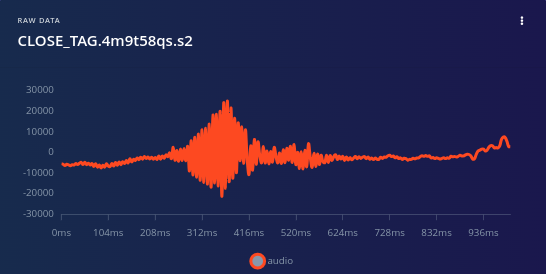
\includegraphics[width=.4\linewidth]{Img/close_tag.png}
    \caption{Espectro señal cierra.}
    \label{close_tag}
    \end{figure}
\item \texttt{NOISE}.
    \begin{figure}[H]
    \centering
    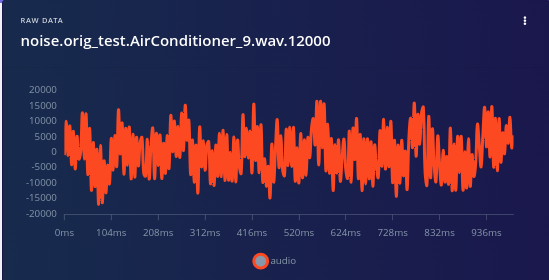
\includegraphics[width=.55\linewidth]{Img/noise.png}
    \caption{Espectro del ruido.}
    \label{noise}
    \end{figure}
\item \texttt{UNKNOWN}.
    \begin{figure}[H]
    \centering
    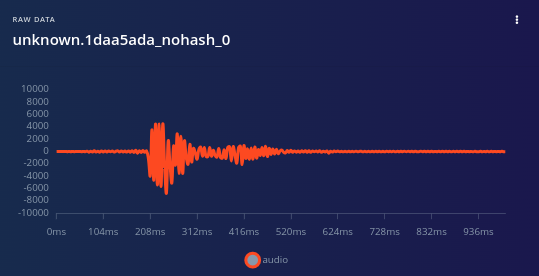
\includegraphics[width=.55\linewidth]{Img/unknown.png}
    \caption{Espectro de sonido desconocido.}
    \label{unk}
    \end{figure}
\end{itemize}
La misma plataforma ayudó a separar las grabaciones de  \SI{20}{\s} en 12 muestras. Lo que hace más rápido y sencillo el procesamiento de datos en las 2 palabras clave. Ahora, las dos etiquetas restantes fueron proporcionadas por Edge-impulse.\\
Luego, con todos los datos listos en \cite{web10} es posible realizar la clasificación de los datos.
    \begin{figure}[H]
    \centering
    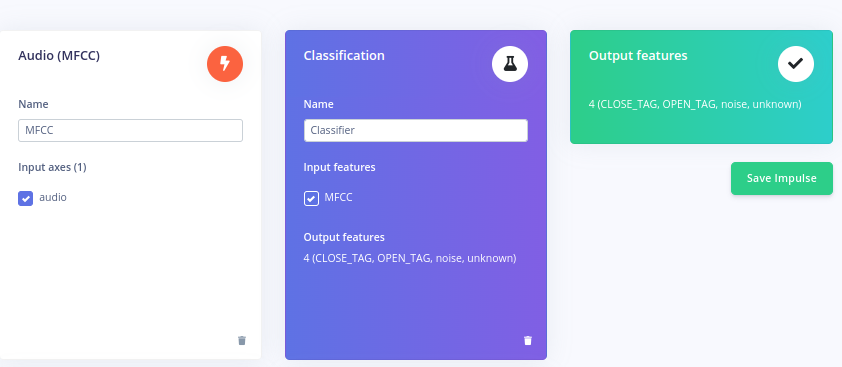
\includegraphics[width=.55\linewidth]{Img/classifier.png}
    \caption{Clasificación de los datos.}
    \label{classi}
    \end{figure}
De donde se usa una técnica de extracción de parámetros: MFCC (Mel-Frequency Cepstral Coefficientes), se definen como coeficientes cepstrales\footnote{se definen como la transformada inversa de Fourier del logaritmo del espectro de la señal de voz.} que se aplican sobre una ventana de tiempo de la señal de voz. Desde el punto de vista matemático es un operador que transforma una convolución en el tiempo en una suma espectral y de esa manera, se logran extraer los dos componentes en una señal de voz: la excitación y el tracto vocal \cite{web9}.\\
Una vez clasificados los datos, los resultados que se obtuvieron fueron los siguientes:
    \begin{figure}[H]
    \centering
    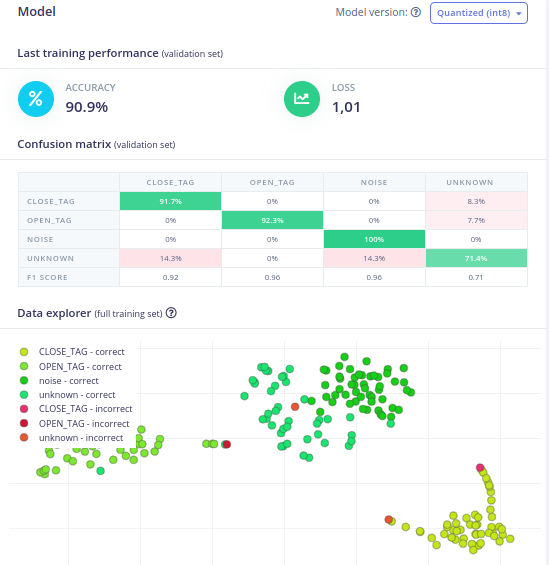
\includegraphics[width=.55\linewidth]{Img/training.png}
    \caption{Resultado fina del entrenamiento.}
    \label{training}
    \end{figure}
Por último, lo que se hizo fue configurar el \texttt{deployment} de todo lo anterior para importarlo a una librería de Arduino. Ya con esto es posible instalarla en el IDE y así editar el código conforme a las necesidades requeridas de acorde a los objetivos plantes. Es decir, que logre reconocer la palabra: \texttt{abrir} y \texttt{cierra} para activar el servomotor y así abrir o cerrar el pica-porte de una puerta, donde habrán unos LEDs que mostrarán el estado del diseño implementado.\par
Una de las primeras pruebas fue editar un poco el código generado y ver como se comportaba cuando escuchaba una de las palabras claves.

\begin{figure}[H]
   \begin{minipage}{0.48\textwidth}
     \centering
    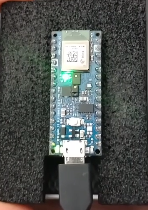
\includegraphics[width=.55\linewidth]{Img/abrir_1.png}
    \caption{Reconocimiento de la palabra abrir.}
    \label{abrir_1}
   \end{minipage}\hfill
   \begin{minipage}{0.48\textwidth}
     \centering
    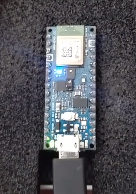
\includegraphics[width=.55\linewidth]{Img/cierra_1.png}
    \caption{Reconocimiento de la palabra cierra.}
    \label{cierra_1}     
   \end{minipage}
\end{figure}
Al decir la palabra abrir y cierra el LED del mcu muestra un color verde y azul respectivamente. También muestra un color rojo al inicio pero esto tiene que ver con la lógica que se tenía implementada.\par
Con esta comprobación fue posible hacer uso del servo motor, implementarle cierta lógica para que éste gire de 0 a 90 grados y viceversa con base al estado en el que se encuentre.
\begin{figure}[H]
   \begin{minipage}{0.48\textwidth}
     \centering
    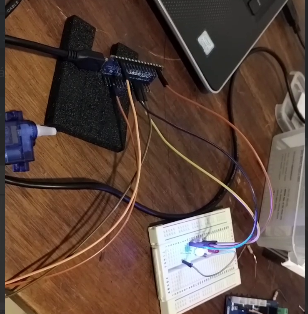
\includegraphics[width=.55\linewidth]{Img/abrir_st.png}
    \caption{Accionamiento del servo con la palabra abrir.}
    \label{abrir_st}
   \end{minipage}\hfill
   \begin{minipage}{0.48\textwidth}
     \centering
    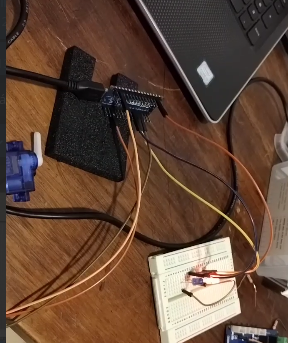
\includegraphics[width=.55\linewidth]{Img/cierra_st.png}
    \caption{Accionamiento del servo con la palabra cierra.}
    \label{cierra_st}     
   \end{minipage}
\end{figure}

Note que:
\begin{itemize}
    \item 0 grados: puerta cerrada.
    \item 90 grados: puerta abierta.
\end{itemize}
\begin{figure}[H]
   \begin{minipage}{0.48\textwidth}
     \centering
    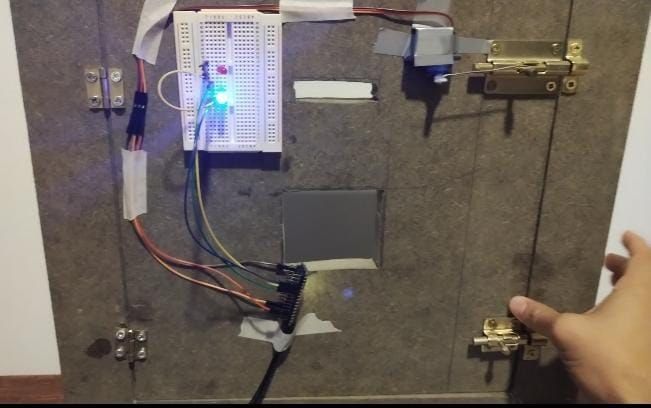
\includegraphics[width=.6\linewidth]{Img/abrir_st2.jpg}
    \caption{Funcionamiento completo con la palabra abrir.}
    \label{abrir_st2}
   \end{minipage}\hfill
   \begin{minipage}{0.48\textwidth}
     \centering
    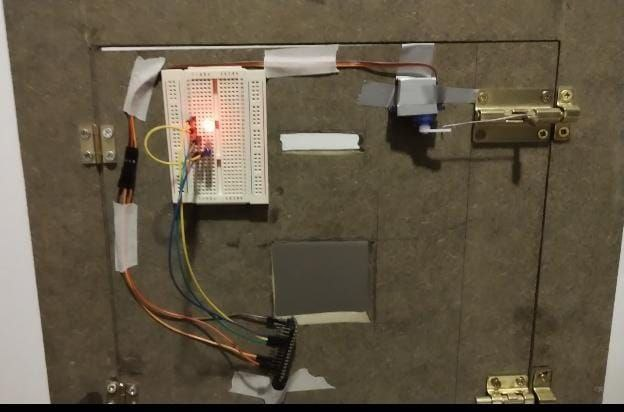
\includegraphics[width=.6\linewidth]{Img/cierra_st2.jpg}
    \caption{Funcionamiento completo con la palabra cierra.}
    \label{cierra_st2}     
   \end{minipage}
\end{figure}
Las imágenes \ref{abrir_st2} y \ref{cierra_st2} muestran el comportamiento esperado. 


%%%%%%  ¡¡¡¡¡ AQUI ME PARECE QUE VA LA SEGUNDA PARTE, FUNCIONAMIENTO COMPLETO ....!!! %%%
Una vez realizado el reconocimiento de voz, se empezó probando todos los componentes electrónicos para verificar su funcionalidad y hacer ejemplos sencillos para entender como trabajar con ellos.
La primera prueba realizada fue las del servo, en el que se utilizó la librería de ''Servo.h'' para poder manejar el mismo, es importante saber que no todos los servos tienen un mismo punto inicial, por lo que para este proyecto se tuvieron que tantear valores para poder trabajarlo de forma correcta.\\
Para el keypad se utiliza la librería de ''Keypad.h'' ya que, simplifica mucho el trabajo, simplemente es de crear una matriz que contenga los caracteres del keypad y hacer un mapeo correcto de los cables para que se detecte el carácter correcto dependiendo del botón que se pulse. Se tuvieron que hacer varias pruebas para determinar como estaba mapeado el keypad.\\
Para el lcd se decidió trabajar con un módulo de I2C, de no ser así la cantidad de cables pasaron de 8 a 4 y gracias a esto solo se tuvo que utilizar la librería de ''LiquidCrystal\_I2C.h'' y se imprimen los mensajes deseados utilizando una comunicación serial mediante el puerto USB.
Todo esto se puede observar en el siguiente enlace.
\url{https://drive.google.com/file/d/1F8vAwWyKLxurYiivwDr2JWspp3p14MrM/view?usp=sharing}
Una vez comprobado el funcionamiento de todo lo utilizado se procedió a ensamblar todo junto con la puerta, el resultado final se observa en las siguientes imagenes:
\begin{figure}[H]
    \centering
    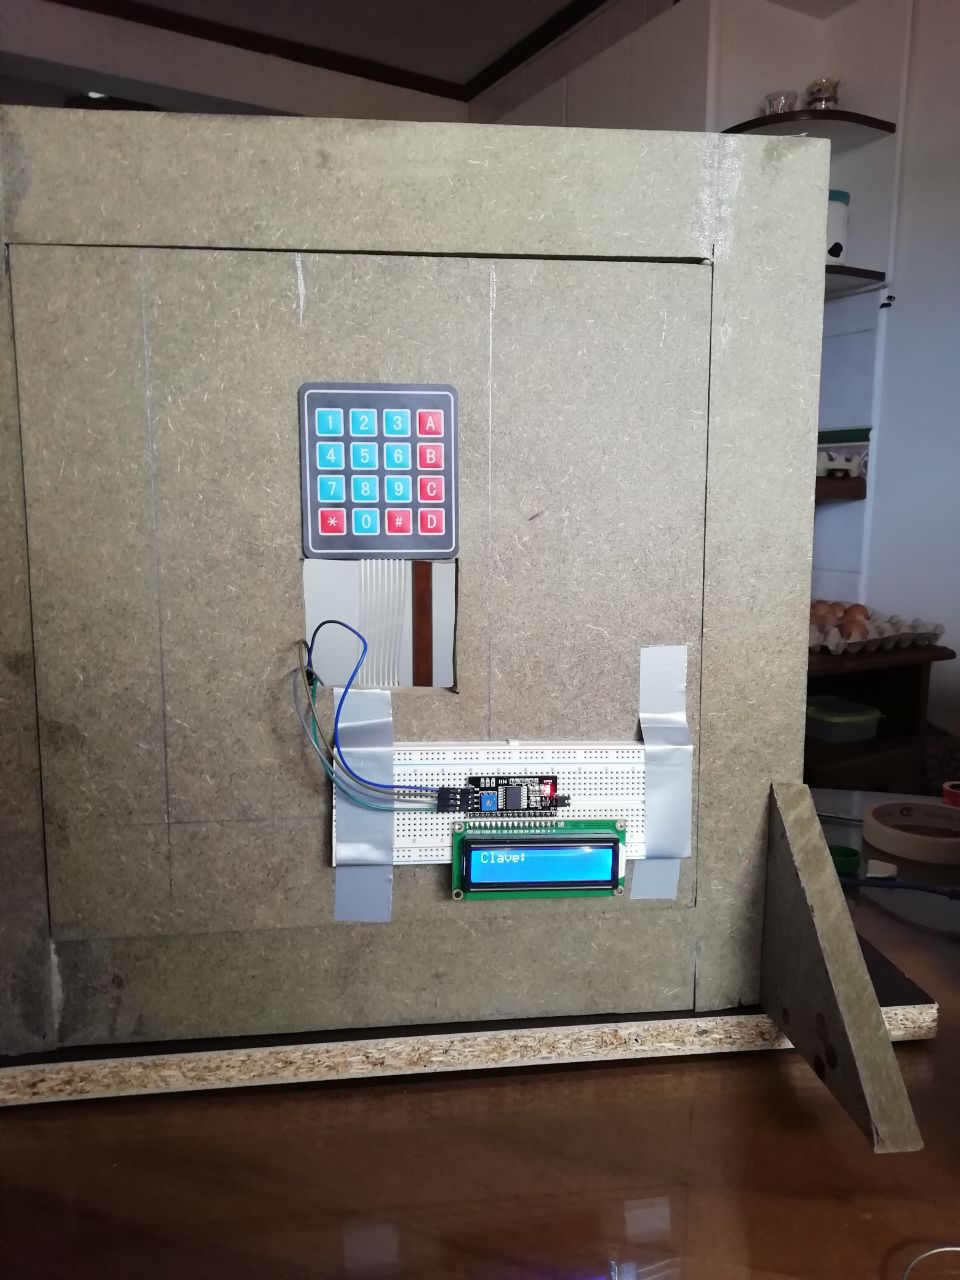
\includegraphics[width=.55\linewidth]{Img/FinalFrente.jpeg}
    \caption{Cerradura final ensamblado parte frontal.}
\end{figure}

\begin{figure}[H]
    \centering
    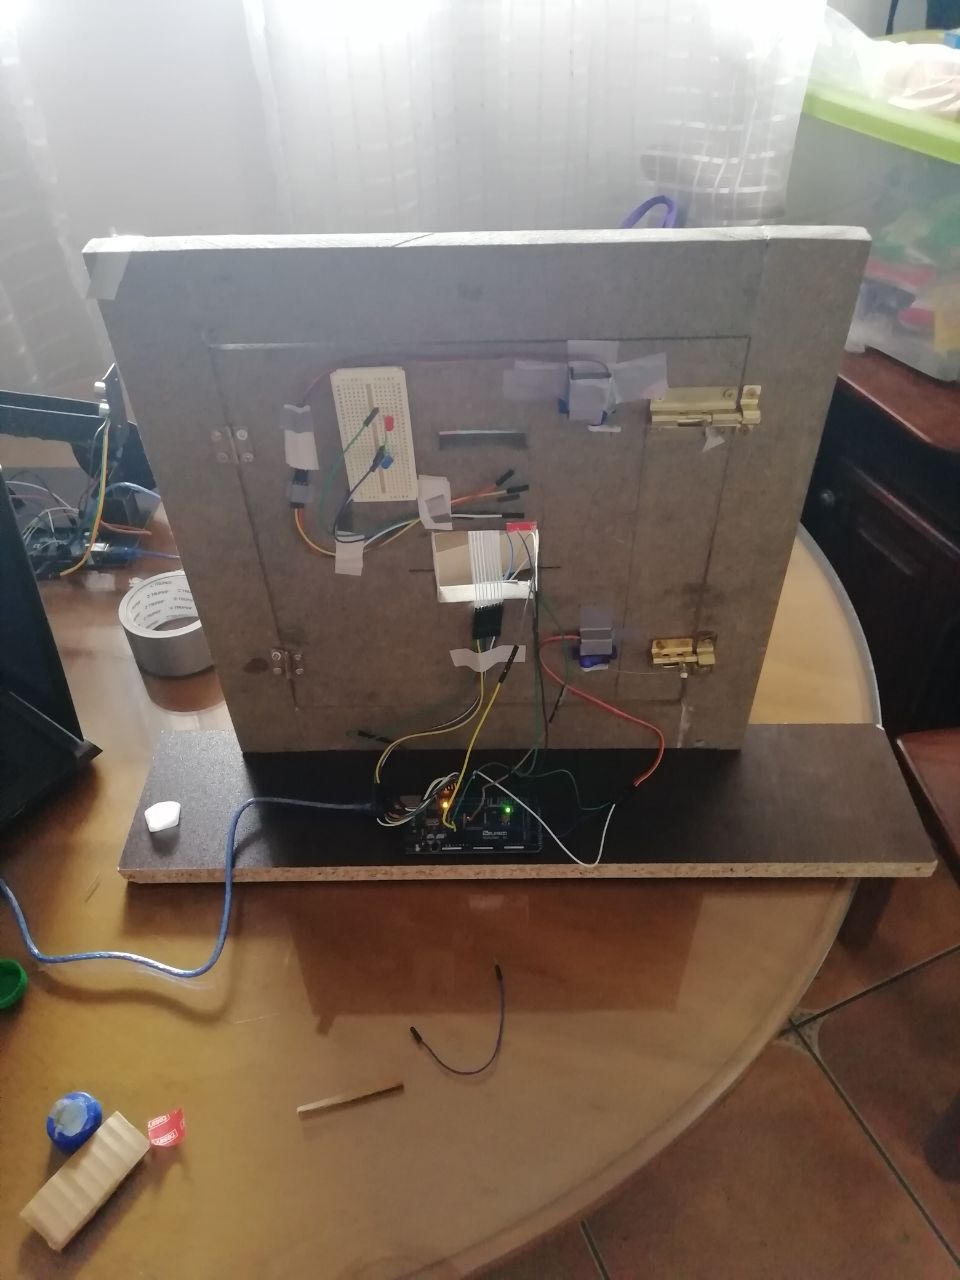
\includegraphics[width=.55\linewidth]{Img/FinalTrasero.jpeg}
    \caption{Cerradura final ensamblado parte trasera.}
\end{figure}




\newpage
\section{Conclusiones y recomendaciones}
A modo de conclusión, es de gran de satisfacción haber realizado un entrenamiento adecuado y así obtener los resultados esperados, es decir, que el microcontrolador logre procesar todas las señales para abrir o cerrar una puerta. Aunque algunas veces el sistema se acciona por si solo, y esto puede ser por ciertas razones, por ejemplo, la cantidad de muestras entrenadas, se esperaba hacer un procesamiento de datos más grandes pero Edge Impulse le costaba cada vez más incluso en repetidas ocasiones el algoritmo detrás de esto excedía el tiempo esperado por lo que terminaba desechar toda la grabación. Por tanto, hay que tener una paciencia (muy pequeña) y poder ver su funcionamiento. Este tipo de proyectos es de carácter muy enriquecedor porque implica mucha investigación, pruebas y errores, los cuales son enseñanzas muy buenas que ayudaron a avanzar en el desarrollo del proyecto. Es increíble la cantidad de proyectos de TinyML que se pueden hacer a partir de lo visto en el curso y lo bueno todo esto que hay muchos recursos para lograrlo.\par

Como recomendaciones:
\begin{itemize}

    \item Comprobar que el funcionamiento de los pines es el correcto, no asumir que todos están buenos y que te lleve a un cambio de planes en el diseño.
    \item Elegir un proyecto que sea realizable y que este de acuerdo a sus conocimientos. Esto por el poco tiempo que se dispone en el tercer ciclo.
    \item Tener mucho cuidado con el manejo de los componentes en todo momento porque causar algún daño en media planificación es muy doloroso por cuestiones de tiempo de más a invertir en la búsqueda del mismo.
    \item  Disfrutar del proceso porque es una etapa de mucho aprendizaje cuando se emprenden nuevos conocimientos sin saber nada.
\end{itemize}

\newpage 

\bibliographystyle{unsrt}
\bibliography{bibliografia.bib}
\newpage

  \section{Anexos}
En esta sección se añade el link del repositorio: \url{https://github.com/JosueC07183/Proyecto-IE0624} y se muestran las hojas del fabricante de los componentes usados para este proyecto. 

\foreach \page in {1,2,3,8,10,11}{
  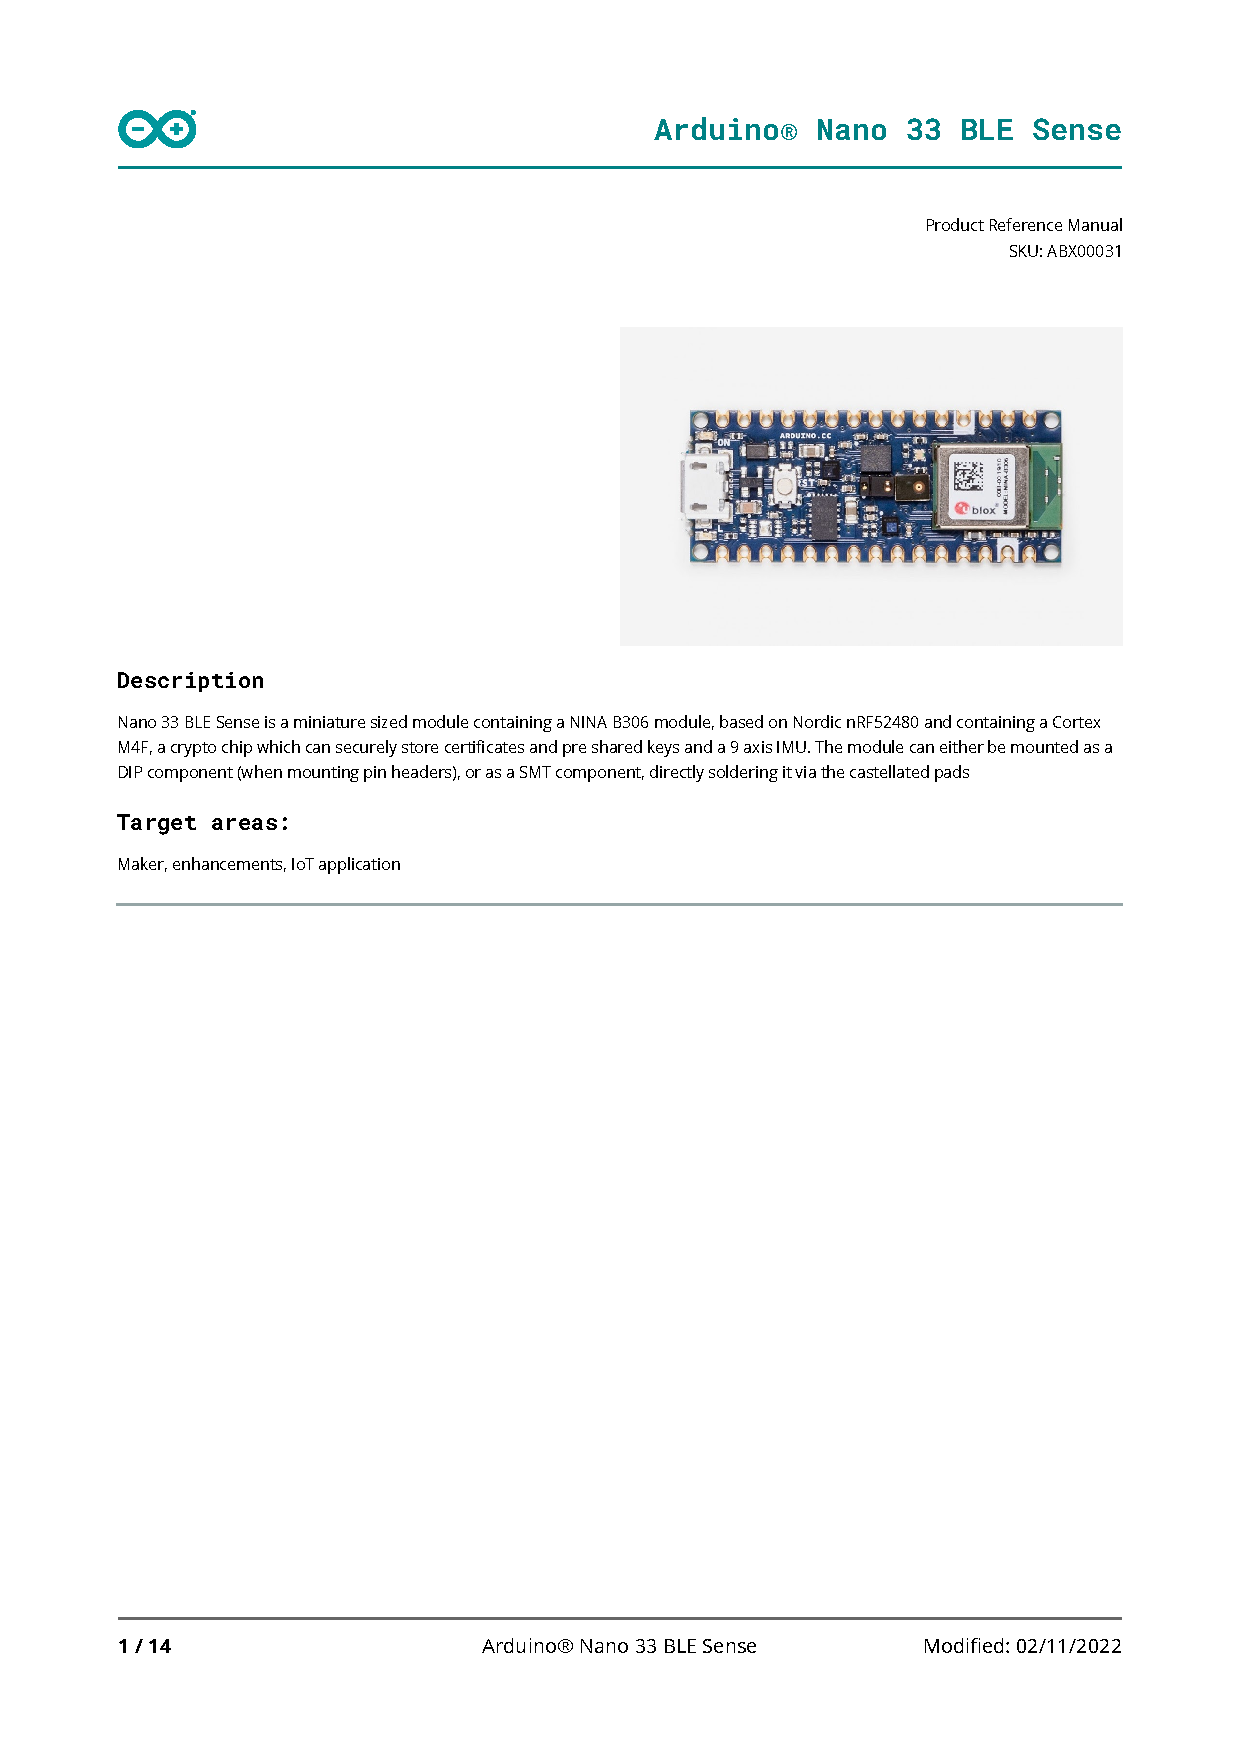
\includepdf[pages=\page]{./Documentos/DatasheetNano33BLE.pdf}
}

\foreach \page in {2,3,9, 10-11}{
  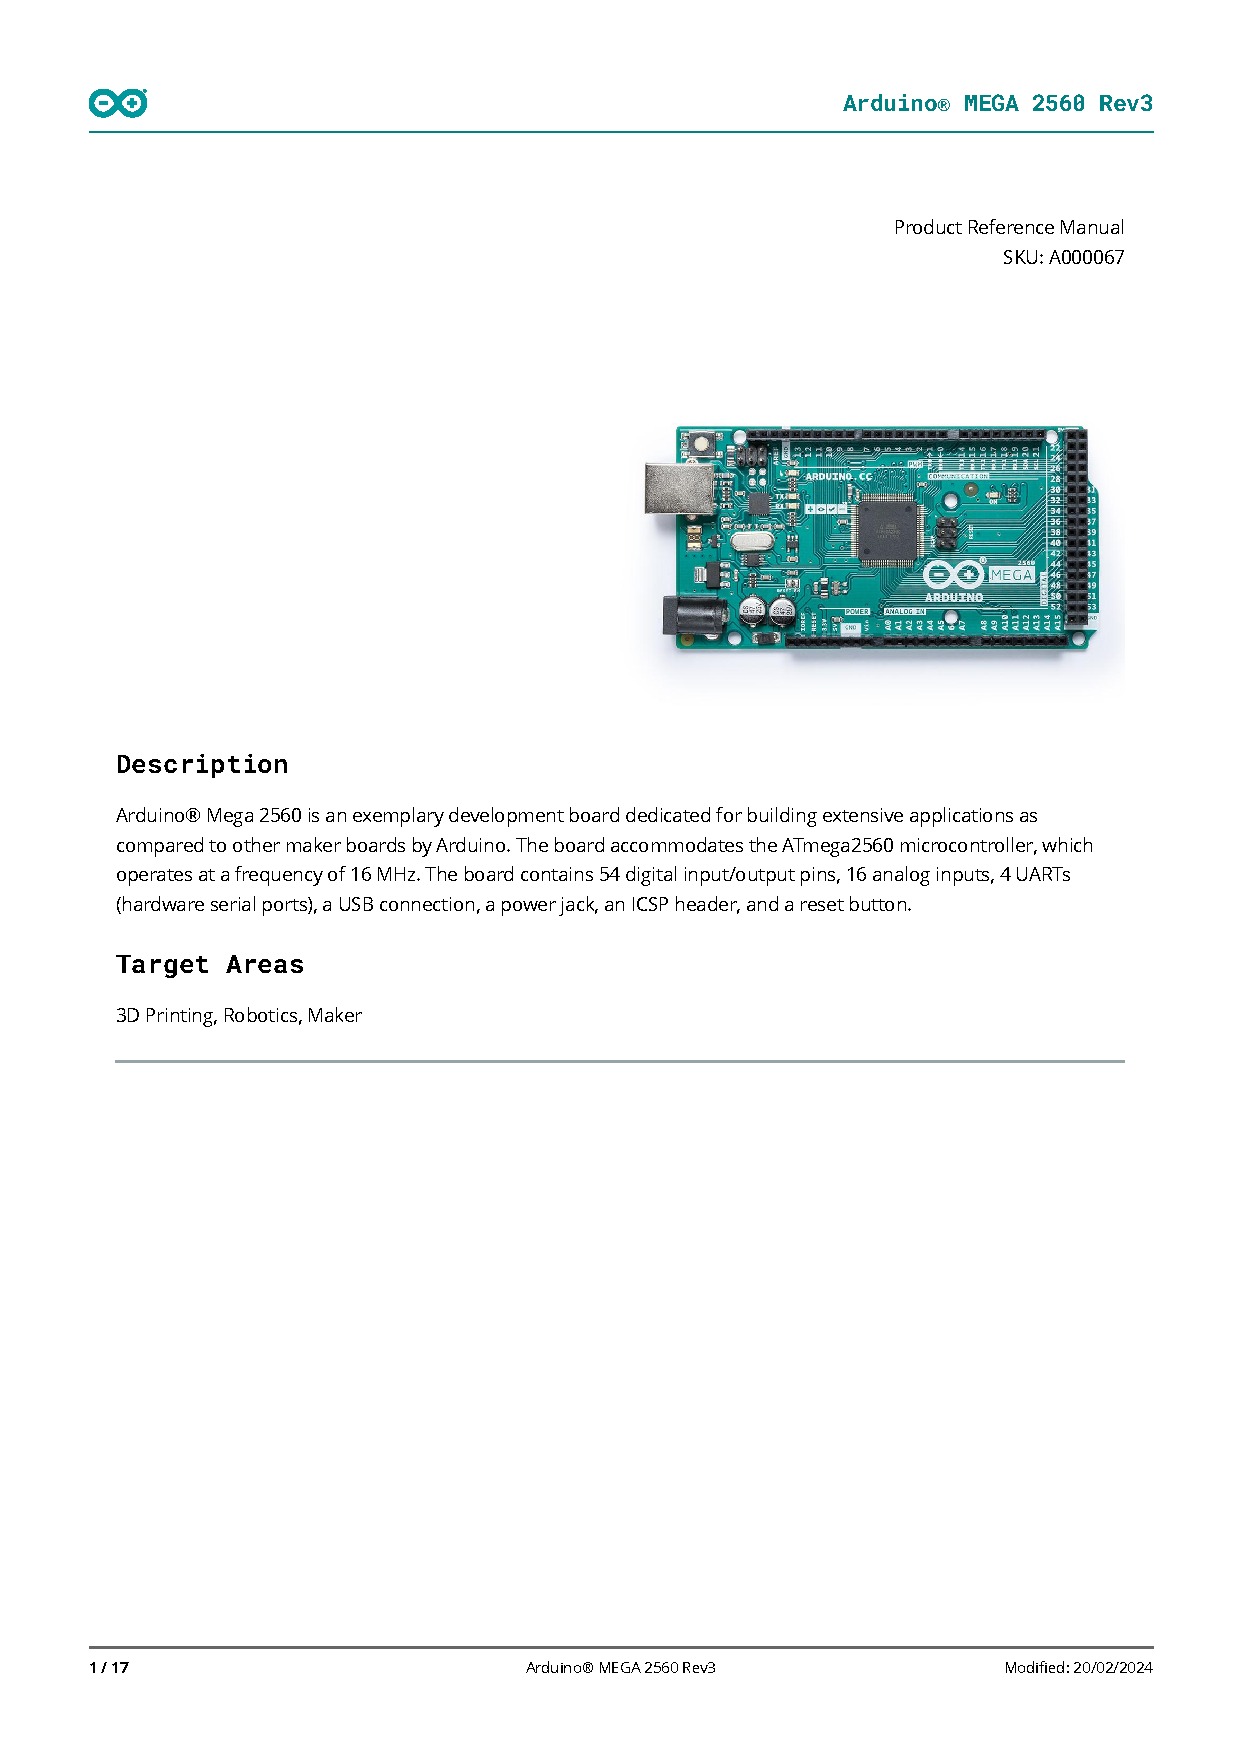
\includepdf[pages=\page]{./Documentos/mega2560datasheet.pdf}
}
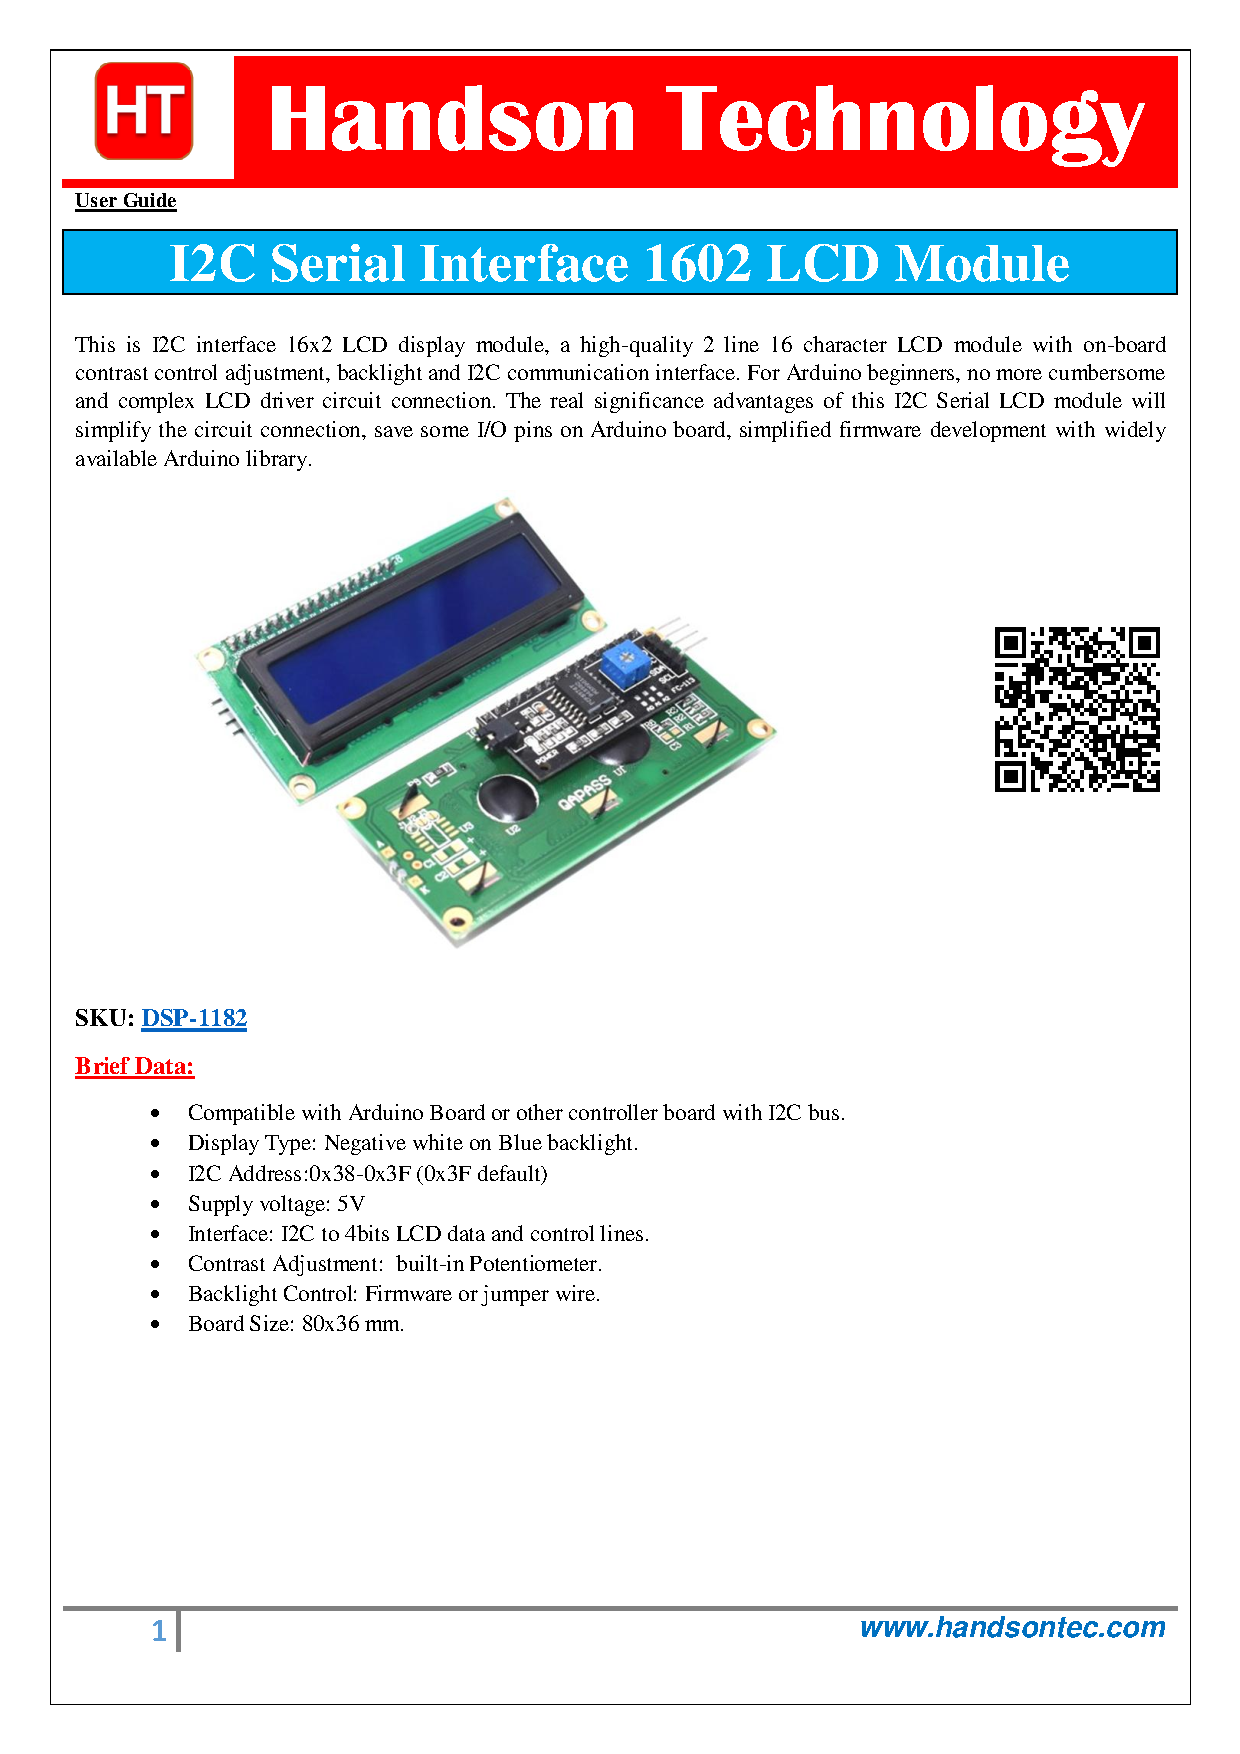
\includepdf[pages=1-3]{./Documentos/i2c_lcd_userguide.pdf}

\foreach \page in {1,3}{
  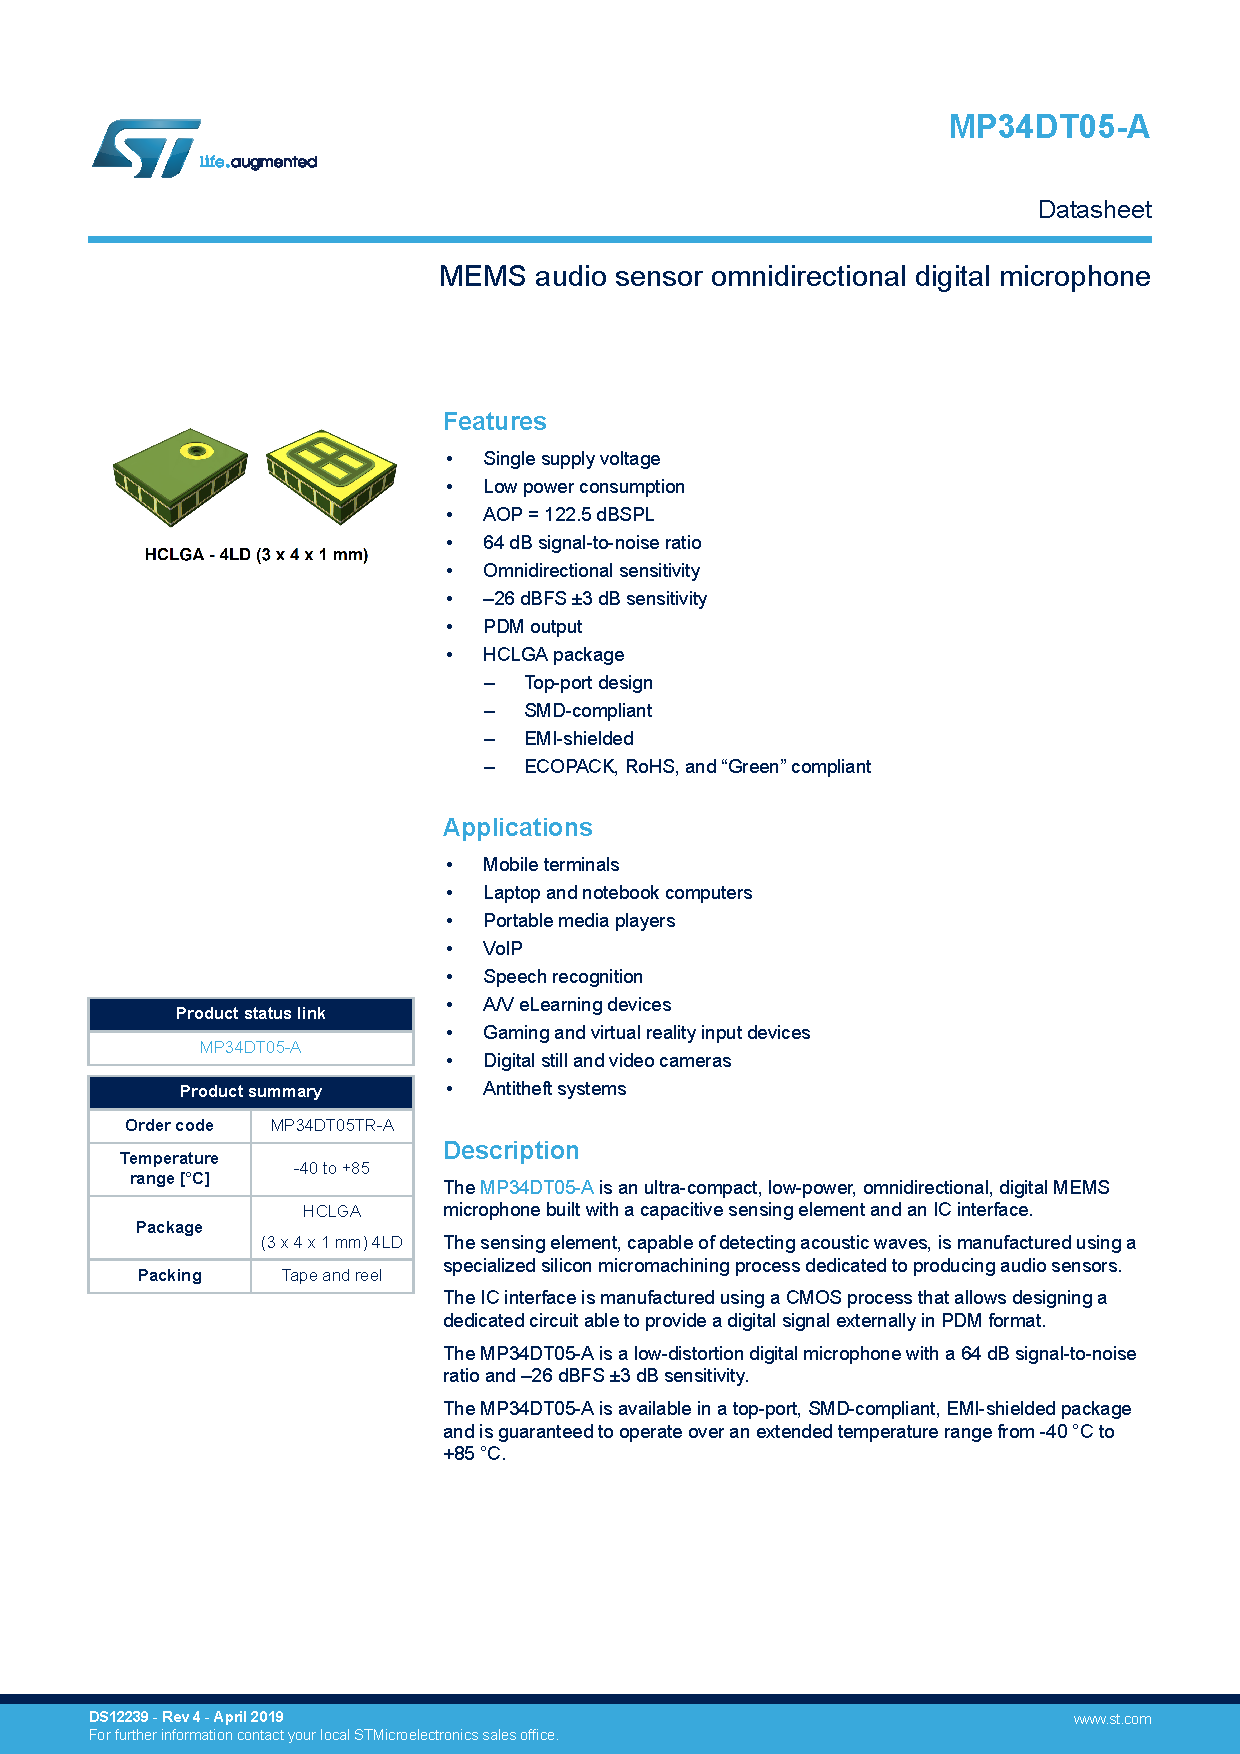
\includepdf[pages=\page]{./Documentos/Nano_BLE_Sense_mp34dt05-a.pdf}
}

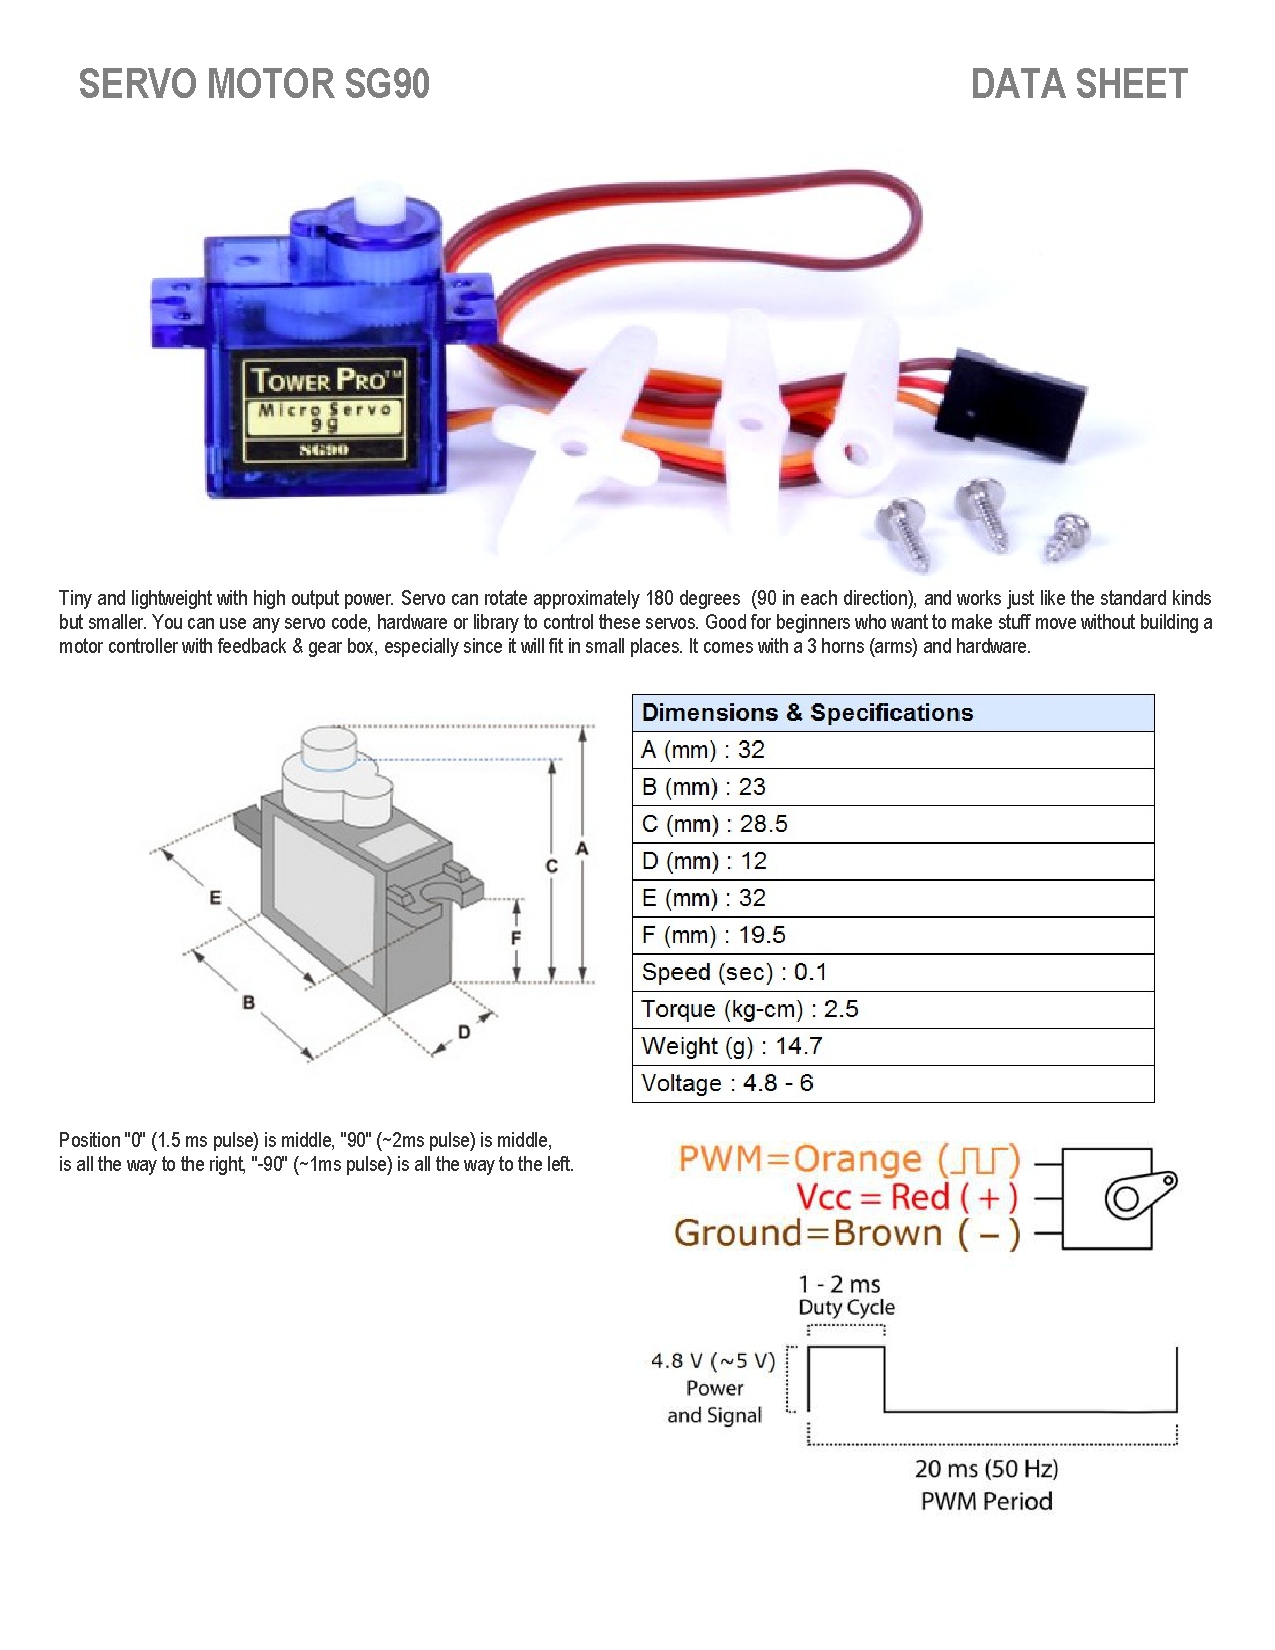
\includepdf[pages=1]{./Documentos/servo_datasheet.pdf}

\end{document}
 

\end{document}